\documentclass[11pt,a4paper]{article}
\usepackage[T1]{fontenc}
\usepackage[utf8]{inputenc}
\usepackage[magyar]{babel}
\usepackage{lmodern}
\usepackage{amsmath,amssymb}
\usepackage{enumitem}
\usepackage{needspace}
\usepackage{tikz}
\usetikzlibrary{arrows.meta,calc}
\usepackage[a4paper,margin=2cm]{geometry}

\pagestyle{empty}
\setlength{\parindent}{0pt}
\setlist[enumerate,1]{label=\textbf{\arabic*.}, leftmargin=*, itemsep=10pt, topsep=3pt}
\setlist[enumerate,2]{label=\alph*), leftmargin=2em, itemsep=4pt, topsep=3pt, parsep=0pt}

% Lencsés képszerkesztés: #1 = f, #2 = t, #3 = tárgymagasság, #4 = xmin, #5 = xmax
\newcommand{\lenskep}[5]{%
  \pgfmathsetmacro{\kk}{1/(1/#1 - 1/#2)}%
  \pgfmathsetmacro{\KK}{-#3*\kk/#2}%
  \pgfmathsetmacro{\HH}{max(#3,abs(\KK))+0.45}%
  \pgfmathtruncatemacro{\virt}{\kk<0 ? 1 : 0}%
  \pgfmathtruncatemacro{\gyujto}{#1>0 ? 1 : 0}%
  \draw[gray!25,very thin] (#4,-3.5) grid (#5,3.5);
  \draw[->,gray] (#4,0) -- (#5,0);
  \ifnum\gyujto=1
    \draw[{Stealth[length=2mm]}-{Stealth[length=2mm]},thick,blue!60!black] (0,-3.5) -- (0,3.5);
  \else
    \draw[{Stealth[length=2mm,reversed]}-{Stealth[length=2mm,reversed]},thick,blue!60!black] (0,-3.5) -- (0,3.5);
  \fi
  \fill (#1,0) circle (1.5pt) node[below,font=\scriptsize] {$F$};
  \fill (-#1,0) circle (1.5pt) node[below,font=\scriptsize] {$F$};
  \draw[very thick,-{Stealth[length=2mm]}] (-#2,0) -- (-#2,#3);
  \begin{scope}
    \clip (#4,-3.5) rectangle (#5,3.5);
    \ifnum\gyujto=1
      \draw[red!75!black] (-#2,#3) -- (0,#3) -- ($(0,#3)!8!(#1,0)$);
    \else
      \draw[red!75!black] (-#2,#3) -- (0,#3) -- ($(0,#3)!-8!(#1,0)$);
    \fi
    \draw[orange!85!black] (-#2,#3) -- ($(-#2,#3)!8!(0,0)$);
    \ifnum\virt=1
      \draw[red!75!black,dashed] (0,#3) -- (\kk,\KK);
      \draw[orange!85!black,dashed] (0,0) -- (\kk,\KK);
      \ifnum\gyujto=0 \draw[red!75!black,dashed] (\kk,\KK) -- (#1,0); \fi
      \draw[very thick,dashed,green!50!black,-{Stealth[length=2mm]}] (\kk,0) -- (\kk,\KK);
    \else
      \draw[violet] (-#2,#3) -- (0,\KK) -- (#5,\KK);
      \draw[very thick,green!50!black,-{Stealth[length=2mm]}] (\kk,0) -- (\kk,\KK);
    \fi
  \end{scope}
}

\begin{document}

\begin{center}
  {\Large\bfseries Geometriai optika -- feladatok -- megoldókulcs}
\end{center}

\begin{enumerate}
\item \textbf{Fénytörés a vízen}
  \begin{enumerate}
    \item $\sin\beta = \dfrac{\sin 50^\circ}{1{,}33} = \dfrac{0{,}766}{1{,}33} = 0{,}576$
      $\Rightarrow$ $\beta \approx 35{,}2^\circ$ (a merőlegeshez törik).\\
      $c_\text{víz} = \dfrac{c}{n} = \dfrac{3\cdot 10^8}{1{,}33} \approx
      2{,}26\cdot 10^8~\tfrac{\text{m}}{\text{s}}$.\\
      A frekvencia nem változik: $f = \dfrac{c}{\lambda} = \dfrac{3\cdot 10^8}{532\cdot 10^{-9}}
      \approx 5{,}64\cdot 10^{14}$~Hz. A hullámhossz a vízben
      $\lambda_\text{víz} = \dfrac{532~\text{nm}}{1{,}33} = 400$~nm.\\
      A búvár is \textbf{zöldnek} látja: a színt a frekvencia határozza meg, nem a hullámhossz
      (ráadásul a szemébe jutva a fény a szem anyagában úgyis ugyanúgy terjed).
    \item A visszavert sugár a merőlegestől $50^\circ$-ra van (felül), a megtört
      $35{,}2^\circ$-ra (alul), a kettő közti szög
      $180^\circ - 50^\circ - 35{,}2^\circ \approx 94{,}8^\circ$.
    \item Vízből levegőbe: $\sin\beta = 1{,}33\cdot\sin 40^\circ = 1{,}33\cdot 0{,}643 = 0{,}855$
      $\Rightarrow$ $\beta \approx 58{,}8^\circ$ (a merőlegestől törik).
  \end{enumerate}

\item \textbf{Lámpa a medence alján}
  \begin{enumerate}
    \item $\sin\alpha_\text{h} = \dfrac{1}{1{,}33} = 0{,}752$ $\Rightarrow$
      $\alpha_\text{h} \approx 48{,}8^\circ$.
    \item A kör szélén éppen határszögben érkezik a fény:
      $r = h\cdot\operatorname{tg}\alpha_\text{h} = 1{,}8~\text{m}\cdot 1{,}14 \approx 2{,}05$~m.
      A körön kívül a beesési szög nagyobb a határszögnél: ott a fény \textbf{teljesen
      visszaverődik} a medencébe.
    \item Ugyanezért a körön kívül a felszín \textbf{tükörként} viselkedik: a búvár a medence
      aljának és falának tükörképét látja. A külvilágot csak egy $2\cdot 48{,}8^\circ \approx
      97{,}5^\circ$-os nyílásszögű kúpon belül, ,,összenyomva'' látja.
  \end{enumerate}

\item \textbf{Prizma a távcsőben}
  \begin{enumerate}
    \item Merőlegesen lép be ($\alpha = 0^\circ$), ekkor $\sin\beta = 0$, nincs irányváltozás.
    \item A fény $45^\circ$-ban éri az átfogót. Az üveg--levegő határszög $41{,}8^\circ$,
      $45^\circ > 41{,}8^\circ$, ezért \textbf{teljes visszaverődés} történik, a fény
      $90^\circ$-kal eltérül, és merőlegesen lép ki az alsó lapon. Feltétel:
      $\sin 45^\circ \ge \dfrac1n$ $\Rightarrow$ $n \ge \sqrt2 \approx 1{,}41$.
    \item Üveg--víz határon: $\sin\alpha_\text{h} = \dfrac{1{,}33}{1{,}5} = 0{,}887$
      $\Rightarrow$ $\alpha_\text{h} \approx 62{,}5^\circ > 45^\circ$: nincs teljes
      visszaverődés, a fény nagy része kilép a vízbe.
      $\sin\beta = \dfrac{1{,}5}{1{,}33}\cdot\sin 45^\circ = 0{,}797$ $\Rightarrow$
      $\beta \approx 52{,}9^\circ$.
    \item A törésmutató függ a színtől (ibolyára a legnagyobb, vörösre a legkisebb), ezért
      ferde beesésnél a színek különböző szögben törnek meg: \textbf{színszóródás}. A
      távcső prizmájában viszont a fény merőlegesen lép be és ki (nincs törés), az átfogón
      pedig visszaverődik, és a visszaverődés törvénye ($\alpha = \alpha'$) nem függ a
      színtől. Így nincs színbontás.
  \end{enumerate}

\newpage
\item \textbf{Képszerkesztés} ($f = 2$~cm, $T = 1{,}5$~cm; piros: párhuzamos sugár,
  narancs: középponton átmenő, lila: fókuszon átmenő sugár, zöld: kép)

  \begin{minipage}[t]{0.49\linewidth}\centering
  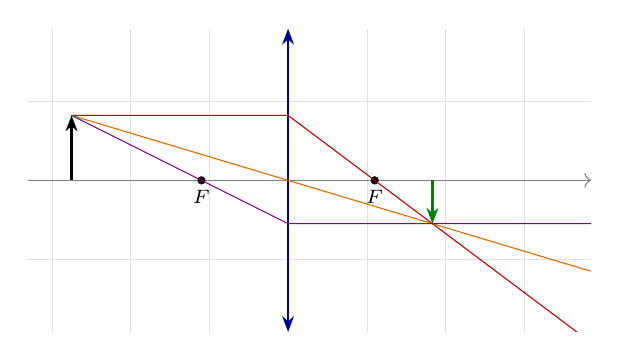
\begin{tikzpicture}[x=0.55cm,y=0.55cm]
    \lenskep{2}{5}{1.5}{-6}{7}
  \end{tikzpicture}\\[2pt]
  \small\textbf{a)} $t = 5$~cm: $\tfrac1k = \tfrac12 - \tfrac15 = \tfrac3{10}$,
  $k \approx 3{,}3$~cm, $N = \tfrac23$, $K = 1$~cm.\\
  Valódi, fordított, kicsinyített.
  \end{minipage}\hfill
  \begin{minipage}[t]{0.49\linewidth}\centering
  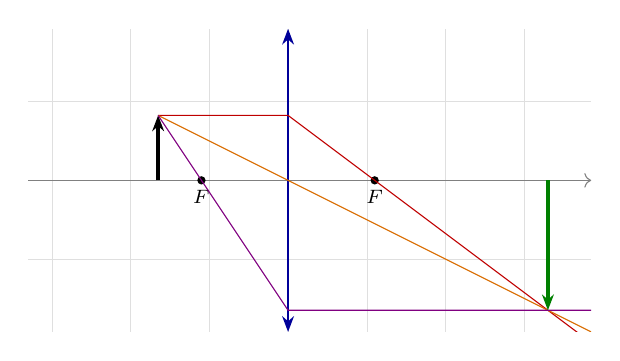
\begin{tikzpicture}[x=0.55cm,y=0.55cm]
    \lenskep{2}{3}{1.5}{-6}{7}
  \end{tikzpicture}\\[2pt]
  \small\textbf{b)} $t = 3$~cm: $\tfrac1k = \tfrac12 - \tfrac13 = \tfrac16$,
  $k = 6$~cm, $N = 2$, $K = 3$~cm.\\
  Valódi, fordított, nagyított.
  \end{minipage}

  \vspace{8pt}
  \begin{minipage}[t]{0.49\linewidth}\centering
  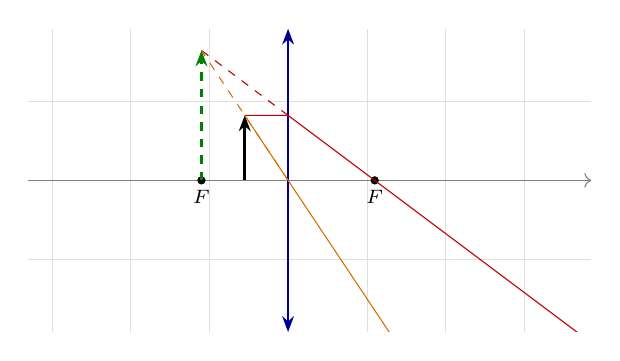
\begin{tikzpicture}[x=0.55cm,y=0.55cm]
    \lenskep{2}{1}{1.5}{-6}{7}
  \end{tikzpicture}\\[2pt]
  \small\textbf{c)} $t = 1$~cm: $\tfrac1k = \tfrac12 - 1 = -\tfrac12$,
  $k = -2$~cm, $N = 2$, $K = 3$~cm.\\
  Látszólagos, egyenes, nagyított (nagyító).
  \end{minipage}\hfill
  \begin{minipage}[t]{0.49\linewidth}\centering
  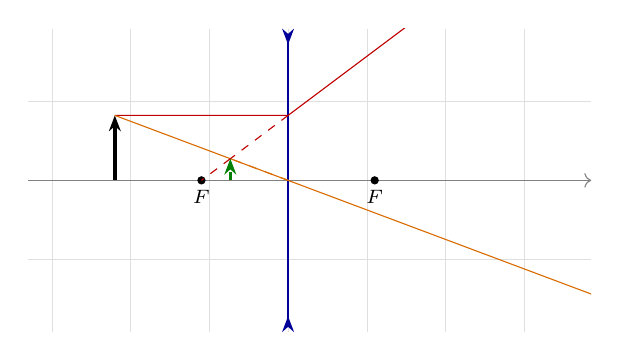
\begin{tikzpicture}[x=0.55cm,y=0.55cm]
    \lenskep{-2}{4}{1.5}{-6}{7}
  \end{tikzpicture}\\[2pt]
  \small\textbf{d)} $f = -2$~cm, $t = 4$~cm: $\tfrac1k = -\tfrac12 - \tfrac14 = -\tfrac34$,
  $k \approx -1{,}33$~cm, $N = \tfrac13$, $K = 0{,}5$~cm.
  Látszólagos, egyenes, kicsinyített.
  \end{minipage}

\item \textbf{Gyűjtőlencse} ($f = 20$~cm, $T = 5$~cm)
  \begin{enumerate}
    \item $D = \dfrac{1}{0{,}2~\text{m}} = 5$~dioptria.
      $\dfrac1k = \dfrac1{20} - \dfrac1{60} = \dfrac1{30}$ $\Rightarrow$ $k = 30$~cm,
      $N = \dfrac{30}{60} = 0{,}5$, $K = 2{,}5$~cm. Valódi, fordított, kicsinyített; az ernyőt
      a lencse túloldalán, $30$~cm-re kell tenni.
    \item $\dfrac1k = \dfrac1{20} - \dfrac1{15} = -\dfrac1{60}$ $\Rightarrow$ $k = -60$~cm,
      $N = \dfrac{60}{15} = 4$, $K = 20$~cm. Látszólagos, egyenes (a tárgy oldalán), ernyőn
      \textbf{nem} fogható fel.
    \item Valódi kép, $k = 4t$: $\dfrac1t + \dfrac1{4t} = \dfrac{5}{4t} = \dfrac1{20}$
      $\Rightarrow$ $t = 25$~cm, $k = 100$~cm. A nagyítás ugyanúgy $4$, de most a tárgy
      $f$ és $2f$ között van, a kép valódi és fordított, és $1$~m-re lévő ernyőn felfogható.
      A b) esetben ($t < f$) a kép látszólagos és egyenes.
    \item Levegőben $\dfrac1f = (n-1)\cdot\dfrac2R$ $\Rightarrow$
      $R = 2(n-1)f = 2\cdot 0{,}5\cdot 20~\text{cm} = 20$~cm.\\
      Vízben a relatív törésmutató $\dfrac{1{,}5}{1{,}33} \approx 1{,}128$:
      $\dfrac1{f_\text{víz}} = 0{,}128\cdot\dfrac{2}{20~\text{cm}} \approx
      0{,}0128~\tfrac1{\text{cm}}$ $\Rightarrow$ $f_\text{víz} \approx 78$~cm.
      Gyűjtőlencse marad ($n_\text{rel} > 1$), csak kb.\ négyszer gyengébb, mert az üveg és a
      víz törésmutatója közel van egymáshoz. (Ezért látunk homályosan a víz alatt búvárszemüveg
      nélkül: a szaruhártya törőképessége a víz mellett nagyrészt elvész.)
    \item A buborékban levegő van, a környezet víz: $n_\text{rel} = \dfrac{1}{1{,}33} < 1$, így
      $n_\text{rel} - 1 < 0$, és pozitív $R$-ek mellett $f < 0$: a domború légbuborék
      \textbf{szórólencse}. (Fordítva: vízben a homorú légrés gyűjt.)
  \end{enumerate}

\item \textbf{Vetítő és fényképezőgép}
  \begin{enumerate}
    \item $\dfrac1t = \dfrac1{10} - \dfrac1{510} = \dfrac{50}{510}$ $\Rightarrow$
      $t = 10{,}2$~cm (alig van a fókuszon túl). $N = \dfrac{510}{10{,}2} = 50$, a kép
      $1{,}2~\text{m} \times 1{,}8~\text{m}$ (fordított, ezért a diát fejjel lefelé tesszük be).
    \item $\dfrac1t = \dfrac1{10} - \dfrac1{310} = \dfrac{30}{310}$ $\Rightarrow$
      $t \approx 10{,}33$~cm: az objektívet kb.\ $1{,}3$~mm-rel \textbf{távolabb} kell vinni
      a diától. $N = \dfrac{310}{10{,}33} = 30$, a kép kisebb:
      $0{,}72~\text{m} \times 1{,}08~\text{m}$.
    \item $\dfrac1k = \dfrac1{50} - \dfrac1{5000} = \dfrac{99}{5000}$ $\Rightarrow$
      $k \approx 50{,}5$~mm. $N = \dfrac{50{,}5}{5000} \approx 0{,}0101$,
      $K \approx 1800~\text{mm}\cdot 0{,}0101 \approx 18{,}2$~mm, tehát ráfér (még fekvő
      formátumban is, $18{,}2 < 24$). Távoli tárgynál $\tfrac1t \approx 0$, ezért
      $k \approx f$: a kép szinte a fókuszsíkban keletkezik.
  \end{enumerate}

\needspace{5\baselineskip}
\item \textbf{Tárgy és ernyő}
  \begin{enumerate}
    \item $t + k = 90$ és $\dfrac1t + \dfrac1k = \dfrac{t+k}{tk} = \dfrac1{20}$
      $\Rightarrow$ $tk = 1800$. Így
      \[ t^2 - 90t + 1800 = 0, \qquad t = \frac{90 \pm \sqrt{8100 - 7200}}{2} = \frac{90 \pm 30}{2}. \]
      $t = 30$~cm ($k = 60$~cm): $N = 2$, nagyított; \quad $t = 60$~cm ($k = 30$~cm):
      $N = 0{,}5$, kicsinyített. (A két helyzet egymás ,,tükörképe'': $t$ és $k$ felcserélődik.)
    \item Általában $t + k = d$, $tk = fd$ $\Rightarrow$ $t^2 - dt + fd = 0$. Valós megoldás
      akkor van, ha $d^2 - 4fd \ge 0$, azaz $d \ge 4f = 80$~cm. Ekkor
      $t = k = 2f = 40$~cm és $N = 1$.
  \end{enumerate}

\item \textbf{Tükrök}
  \begin{enumerate}
    \item $f = R/2 = 30$~cm. $t = 20$~cm: $\dfrac1k = \dfrac1{30} - \dfrac1{20} = -\dfrac1{60}$
      $\Rightarrow$ $k = -60$~cm, $N = 3$: látszólagos, egyenes, háromszorosan nagyított kép
      (a tükör ,,mögött''). $t = 40$~cm-nél már a fókuszon kívül vagyunk:
      $\dfrac1k = \dfrac1{30} - \dfrac1{40} = \dfrac1{120}$, $k = 120$~cm, a kép valódi és
      fordított, és a fejünk mögött keletkezik, ezért csak elmosódott foltot látunk. A
      kozmetikai tükör tehát csak $f$-en belül működik.
    \item $f = -0{,}5$~m. $\dfrac1k = -\dfrac1{0{,}5} - \dfrac1{10} = -2{,}1~\tfrac1{\text{m}}$
      $\Rightarrow$ $k \approx -0{,}48$~m (a tükör mögött, közel a fókuszhoz).
      $N = \dfrac{0{,}476}{10} \approx 0{,}048$, $K \approx 4{,}5~\text{m}\cdot 0{,}048
      \approx 21$~cm. Látszólagos, egyenes, kicsinyített. A domború tükör sokkal nagyobb
      \textbf{látószöget} fog át, mint a síktükör, így az egész kereszteződés belefér (cserébe
      a tárgyak kisebbnek és távolabbinak tűnnek).
    \item A síktükör képe a tükör mögött ugyanolyan messze van, mint a tárgy előtte, és
      ugyanakkora. A talpról a szembe jutó sugár a tükröt a talp és a szem közti magasság
      felénél éri, a fejtetőről érkező a fejtető és a szem közti magasság felénél. A
      szükséges tükörhossz így a testmagasság fele: \textbf{$85$~cm}, és ez \textbf{nem
      függ} a távolságtól (a tükör alsó széle a szemmagasság felénél legyen).
  \end{enumerate}

\item \textbf{A szem és a szemüveg}
  \begin{enumerate}
    \item A végtelen távoli tárgyról $40$~cm-re lévő látszólagos kép kell:
      $\dfrac1f = 0 + \dfrac1{-0{,}4~\text{m}}$ $\Rightarrow$ $f = -40$~cm,
      $D = -2{,}5$~dioptria: \textbf{szórólencse}.
    \item $t = 0{,}25$~m, $k = -1$~m: $\dfrac1f = \dfrac1{0{,}25} - \dfrac11 = 3~\tfrac1{\text{m}}$
      $\Rightarrow$ $D = +3$~dioptria, $f \approx 33$~cm: \textbf{gyűjtőlencse}.
    \item $k = -25$~cm: $\dfrac1t = \dfrac15 + \dfrac1{25} = \dfrac6{25}$ $\Rightarrow$
      $t \approx 4{,}2$~cm (a fókuszon belül), $N = \dfrac{25}{4{,}17} = 6$.
  \end{enumerate}

\item \textbf{Szóbeli tétel -- mintaválaszok}

  \textbf{(A) A fénytörés.} Homogén közegben a fény egyenes vonalban terjed. Két közeg
  határán egy része visszaverődik (a beesési szög egyenlő a visszaverődési szöggel), más része
  megtörik, azaz megváltoztatja az irányát. A törés oka, hogy a fény terjedési sebessége a két
  közegben különböző. Az abszolút törésmutató $n = c/c_\text{közeg}$, ez a vákuumra $1$, a
  vízre $1{,}33$, az üvegre kb.\ $1{,}5$. A Snellius--Descartes-törvény szerint
  $\sin\alpha/\sin\beta = c_1/c_2 = n_2/n_1$, a szögeket a beesési merőlegestől mérjük, és a
  beeső sugár, a megtört sugár és a merőleges egy síkban van. Optikailag sűrűbb közegbe
  lépve a fény a merőlegeshez törik. Töréskor a frekvencia nem változik, a hullámhossz
  $n$-ed részére csökken. Ha a fény sűrűbb közegből ritkább felé halad, a merőlegestől törik,
  és ha a beesési szög eléri a határszöget ($\sin\alpha_\text{h} = n_2/n_1$), a megtört sugár
  a felület mentén halad. Ennél nagyobb szögnél teljes visszaverődés lép fel, ezt használja
  az optikai szál, a prizmás távcső, és ettől csillog a gyémánt. A törésmutató függ a
  színtől is (színszóródás): az ibolya fény törik a legjobban, ezért bontja színekre a
  prizma a fehér fényt, és ezért keletkezik szivárvány. Hétköznapi példa még a vízbe
  dugott, ,,megtörtnek'' látszó kanál és a valóságosnál sekélyebbnek látszó medence.

  \textbf{(B) Leképezés lencsékkel és gömbtükrökben.} A gyűjtőlencse és a homorú tükör a
  tengellyel párhuzamos sugarakat a fókuszpontba gyűjti ($f > 0$), a szórólencse és a domború
  tükör úgy szórja szét őket, mintha a fókuszból jönnének ($f < 0$). Gömbtükörnél $f = R/2$,
  a lencse erősségét dioptriában adjuk meg: $D = 1/f$. A képet nevezetes sugármenetekkel
  szerkesztjük: a párhuzamos sugár a fókuszon át halad tovább, az optikai középponton átmenő
  sugár nem törik meg, a fókuszon átmenő sugár párhuzamos lesz. Ha a sugarak valóban
  találkoznak, valódi képet kapunk, ez ernyőn felfogható. Ha csak a meghosszabbításaik
  találkoznak, a kép látszólagos. A leképezési törvény $1/f = 1/t + 1/k$, a nagyítás
  $N = K/T = |k|/t$. Gyűjtőlencsénél $t > 2f$ esetén valódi, fordított, kicsinyített kép
  keletkezik (fényképezőgép, szem), $f < t < 2f$ esetén nagyított (vetítő), $t < f$ esetén
  látszólagos, egyenes, nagyított (nagyító). A szórólencse mindig látszólagos, egyenes,
  kicsinyített képet ad. A szemben a retinán valódi, fordított, kicsinyített kép keletkezik,
  az élességet a szemlencse fókusztávolságának változtatása állítja be (alkalmazkodás). A
  rövidlátást szórólencsével, a távollátást gyűjtőlencsével javítjuk. A mikroszkóp és a
  csillagászati távcső két gyűjtőlencséből áll: az objektív valódi képét az okulárral, mint
  nagyítóval nézzük.

  \medskip
  \textbf{Szempontok:} pontos fogalmak (törésmutató, határszög, fókusztávolság, valódi és
  látszólagos kép); a legfontosabb összefüggések (törési törvény, $\sin\alpha_\text{h}$,
  leképezési törvény, nagyítás, dioptria); legalább egy rajz (törés vagy képszerkesztés) és
  egy-egy hétköznapi alkalmazás; összefüggő, logikus felépítés.
\end{enumerate}

\end{document}
